\section{Task, data and representation}
Given an observed log prefix from one machine, the model predicts a distribution over 14 next-event classes. The release contains complete histories for 6,500 training systems and truncated histories for 900 test systems \cite{brief}. Each observed row includes an event identity, timestamp, contextual fields and numerical measurements. We sort by event index within each system and form the label from the first event after the cutoff.

\IfFileExists{tables/data_summary.tex}{In the fitting split, RECOVERY is the most frequent event (26.5\%) and CONTROL\_ALERT is the least frequent (1.0\%). The median gap between consecutive events is 0.96 timestamp units and the 95th percentile is 2.93. The highest missing fraction is 1.6\% for vibration\_reading.
}{
\todo{Summarize the fitting split's class imbalance, sensor missingness and inter-event gaps using the EDA outputs.}}
\IfFileExists{figures/eventflow_eda.pdf}{
\begin{figure}[htbp]
\centering
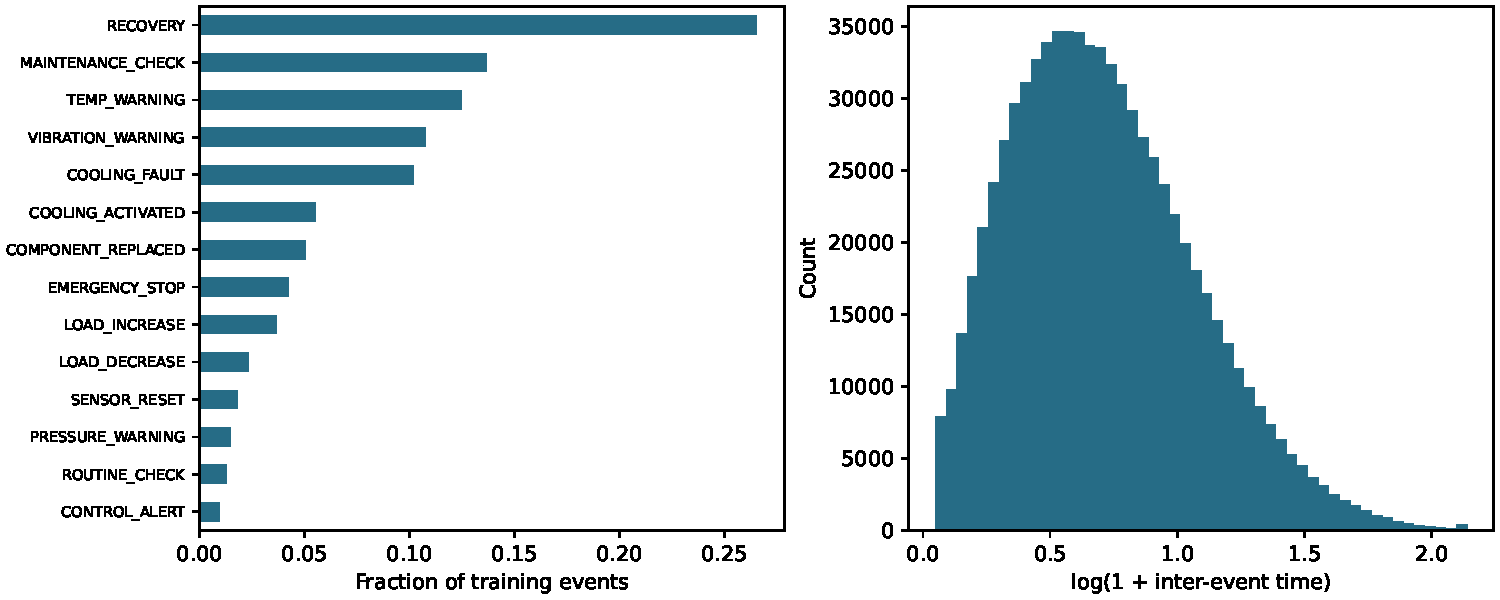
\includegraphics[width=0.88\linewidth]{figures/eventflow_eda.pdf}
\caption{Event frequency and inter-event gap distribution within fitting systems.}
\end{figure}}{}

\begin{table}[htbp]
\centering\small
\begin{tabularx}{\linewidth}{@{}lX@{}}
\toprule
Feature group & Representation and motivation \\
\midrule
Current record & Latest event, context and measurements capture the machine state at the cutoff. \\
Event order & The previous six events and the final event pair represent short transition motifs. \\
Event counts & Per-class counts over the last 8, 32 and 90 events measure recent prevalence at different scales. \\
Timing & Recent log-transformed gaps and elapsed time since each event represent bursts and recency. A type unseen in the prefix has missing recency. \\
Sensor history & Trailing means and least-squares slopes over 8 and 32 events represent levels and trends. Slopes use event positions and skip missing values. \\
\bottomrule
\end{tabularx}
\caption{Classical features grouped for ablations.}
\end{table}
The fitting split shows positive correlations between the main and secondary temperature probes ($r=0.61$) and between the vibration probes ($r=0.79$). The secondary temperature probe also changes more between successive records (median absolute change 0.090 versus 0.056). These differences suggest testing whether trailing means and slopes add information beyond a single reading. Observed variation combines actual changes in system state with possible measurement noise.
